
Because we expect you to be following along actively, we're not going to spend several chapters on theory before you get to do anything fun. Instead, we're going to get you writing code and testing it on your Arduino right away. And, we're going to start you with the simplest, and possibly most important, program you can write using \plumbing.

\GOALS
The goals for this chapter are for you to:

\begin{enumerate}
	\item Write your first program using the \plumbing library.
	\item Run it on your Arduino.
	\item Break your first program, and fix it.
\end{enumerate}


\section{Step By Step}
In most chapters, we would now dive straight into the code you need to write or the circuit you need to build, and then discuss the patterns you should be aware of in the program you just wrote. (Programs have many patterns to them---learning to recognize these patterns is an important step in becoming comfortable with programming in any language.) In this chapter, we'll take it slow and go one step at a time.
          
\subsection{Open JEdit}
JEdit is a free and open-source editor written in Java. It runs on Mac, Linux, and Windows. We added a ``plug-in'' to this project that lets JEdit talk to your Arduino. You can freely download a version of JEdit from \ccc that has our plug-in pre-configured and ready to go for your choice of operating system.
      
\begin{figure}[bph]
  \begin{center}
    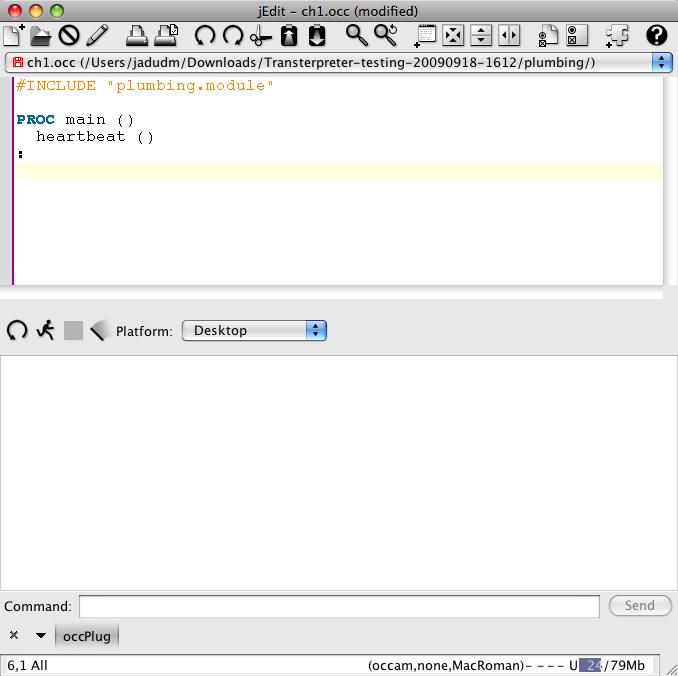
\includegraphics[height=2.5in]{screenshots/20091207-jedit-docked-occplug}
    \caption{The JEdit program editor.}
    \label{screenshot:jedit-occplug-docked}
  \end{center}
\end{figure}

\afterpage{\clearpage}

\subsection{Write your Program}
Once you have JEdit open, you can write your first program. The first step is to get the built-in LED on your Arduino blinking---this will tell us that everything works. 

%\CODE
\lstinputlisting[%caption=The {\code heartbeat} should always be beating.,
label=code:heartbeat]{code/heartbeat.occ}

Type the above program into JEdit. Note that there are some spaces hidden there. Here's the same program, but with the spaces clearly marked:

%\CODE
\lstinputlisting[%caption=The {\code heartbeat} with spaces shown.,
label=code:heartbeat,showspaces=true]{code/heartbeat.occ}

Those {\strong spaces matter a lot}. The most important spaces are the ones on the left-hand side of each line---the {\strong indentation}. If you get indentation wrong in \occam, you'll get an error. We'll explore some common errors at the end of the chapter. 

After copying the code, save it as {\code heartbeat.occ}. If you'd like to call it something else, please feel free to do so. On the Mac, you can press COMMAND-S, and under Linux and Windows, CTRL-S. Or, you can click the little floppy disk in the toolbar. Regardless of how you do it, save your work often!

% XXX Need to tell them to "Setup Arduino," which requires downloading the TVM...

\subsection{Build Your Code}
Your code is human-readable. (You may not feel that way yet, but it is.) We need to convert it from something you understand to something your Arduino understands. We would properly call this {\em compiling} your program. Go up to the {\em Plugins} menu, go down to {\em Plumbing}, and select the {\em Start Plumbing} option. You'll get a new floating window that provides a few critical tools. First, you need to select ``Arduino'' from the drop-down menu (it defaults to ``Desktop'').

% XXX Need to get a version of this image that has "Arduino" instead of "Desktop"       
\begin{figure}[h]
  \begin{center}
    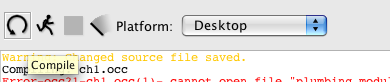
\includegraphics[width=0.8\linewidth]{screenshots/20091207-compile-button}
    \caption{Compile your code before uploading.}
    \label{screenshot:compile-button}
  \end{center}
\end{figure}

Once you have the Plumbing extension running, you can compile and run your program. When you press the round arrow, our tools first check to see if your code is grammatically correct, and then transform your code into something that will run on the Arduino. If you made any mistakes in typing in your program, this is where you'll get one or more seemingly incomprehensible errors. Think of them not as ``errors'' but instead as ``learning opportunities.''
                                         
% XXX Need to cover how we select which Arduino in the plugin...
If you code compiled, you're good to go! Hit the running figure, and your code will be sent to your Arduino and begin executing.

\PATTERNS
When you're learning to program, it is important to see the patterns that exist in the code. Sometimes these patterns are strict rules that you cannot violate, or you will encounter an error. We will also see patterns that represent how programmers typically do things.\footnote{Should we differentiate in the book more clearly?} We'll try and mention when we're introducing one and not the other, but really we expect you to discover which are which through careful experimentation.

\subsection{The \PROCedure Definition}
The first pattern you see in this program is the definition of the procedure {\code main}. Lets look at that pattern again (Figure~\vref{pattern:proc-defn}).

\begin{figure}[h]
  \begin{center}
    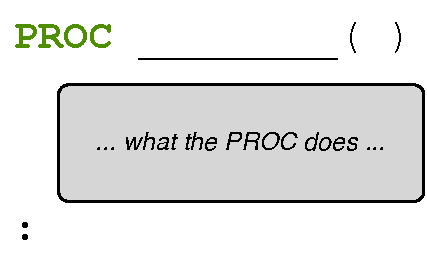
\includegraphics[scale=1.0]{images/ch1-proc-defn-pattern}
    \caption{A procedure definition.}
    \label{pattern:ch1-proc-defn}
  \end{center}
\end{figure}

You will see a lot of \PROCedure definitions while you are using \plumbing, because they help us keep our code organized. A \PROCedure definition always starts with the word \PROC. This is followed by the name of the procedure; in our first program, the procedure is called {\code main}. A set of parentheses come next, and then we hit return. (We'll learn where and when to put things inside those parentheses later!) We will call the stuff inside the \PROCedure its ``body.'' This is the code that makes up the actions of the \PROC we are writing. Note that the body must be indented two spaces. 

The \PROC ends with a colon, all by itself on a line. This signals that we're done defining this particular \PROC, and are ready to start writing another. We'll get to that in Chapter \XXX.

\subsection{A \PROCedure Call}
Look again at line 2 of our first program:

\lstinputlisting[]{code/heartbeat.occ}

From what we have just learned about \PROC definitions, we can say that the body of the \PROC named {\code main} is one line long. That line is a \PROCedure call. A procedure call typically looks like Figure~\vref{pattern:proc-call}.

\begin{figure}[h!]
  \begin{center}
    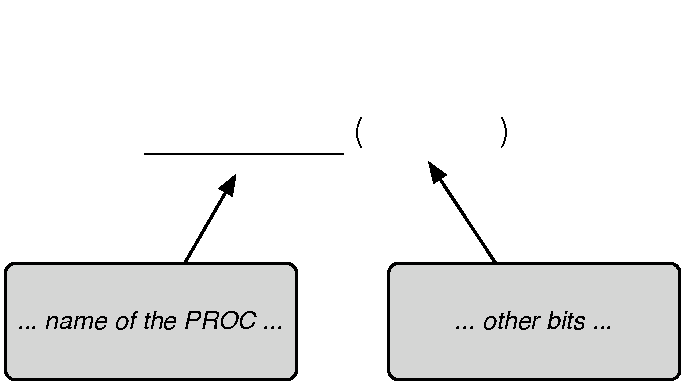
\includegraphics[width=\linewidth]{images/ch1-proc-call-pattern}
    \caption{A procedure call.}
    \label{pattern:ch1-proc-call}
  \end{center}
\end{figure}

A procedure call is a way of saying ``someone else wrote a bunch of great code, and I'd like to use it here, please.'' In this case, we wrote a \PROC called {\code heartbeat}, and we're making it available for you to use. That code blinks the LED on the Arduino.\footnote{You will learn how to write everything we show you in the first ten chapters, so you'll get to see all of the magic soon enough.} We would say that the \PROC called {\code heartbeat} is part of the \plumbing library. Or, if you prefer, when you are programming using \plumbing, {\code heartbeat} is one of the procedures provided for you to use.

\BREAKAGE
With every new piece of code or pattern, there are a dozen ways to break it. Because we want you to be {\em empowered explorers}, we're going to help you break your code at the end of every chapter. We highly recommend you experiment not only with writing programs that work, but also with writing programs that {\strong do not} work. You should keep a notebook of how you break these programs; while it may seem easy to fix them now, you may become confused when you decide to tackle a program of your own design, later.

\begin{description}
  \item[Misspellings]\ \\ One of the most common errors made by beginning programmers in any language are typos and misspellings. What happens if you type {\code PRC} instead of {\code PROC}? {\code maim} instead of {\code main}? {\code hearbeat} instead of {\code heartbeat}?

	\item[CAPS LOCK]\ \\ What happens if you write {\code proc} instead of {\code PROC}? Likewise, {\code Heartbeat} instead of {\code heartbeat}? Problems with capitalization are common in all programming languages.

	\item[Forget the colon]\ \\ What happens when you leave the colon off the end of a \PROC definition? This is a  common error.
	
	\item[Forget the parens, I]\ \\ What happens when you leave one or both of the parentheses off the \PROC definition?
	
	\item[Forget the parens, II]\ \\ What happens when you leave one or both of the parentheses off the \PROC call in the body?
	
	\item[Indentation]\ \\ What happens if you indent the body of the \PROC by one space instead of two? Three spaces? 
\end{description}

\subsection{Programming Strategies}
Remember, learning to program in any language can be a frustrating experience. We highly recommend a few strategies for helping get over any hurdles you might encounter:

\begin{description}
	\item[Community]\ \\ We have a website with more information and mailing lists you can join; take a look at \url{http://concurrency.cc/}. If you get stuck, join the discussion list and ask a question. We're there to help.
	\item[Attention to Detail]\ \\ Spaces matter in \plumbing, and they are {\em invisible}. Be careful about what you do, and begin learning to look with the eyes of a programmer: start looking for patterns and the invisible parts of your code.
	\item[Take Notes]\ \\ As you discover new kinds of mistakes you've made, take the time to make note of them, as well as your analysis of how you fixed them. Eventually, you won't need to make the notes, because you'll make fewer mistakes.
	\item[Take Breaks]\ \\ While programming and hacking are fun, sometimes you can get stuck. Walk away. Talk to an old friend on the phone. Do something else, and let your mind work on the problem in a different space.
\end{description}

\EXPLORATIONS
This chapter had a lot of background material in it, but that is to be expected: it is the first chapter. And, because our code was so simple, there aren't a lot of explorations you can do yet. We promise, there will be more later.

\begin{itemize}
	\item What happens if you unplug the USB cable powering your Arduino while the program is running? 
	\item What happens when you plug it back in?
	\item What happens if you press the reset button while your program is running?
\end{itemize}
